\documentclass[5pt]{article}
\usepackage{mathptmx,amsmath}
\usepackage{pdfslide2,pause}
\usepackage{eurosym}
\usepackage[portuguese,english]{babel}
%\usepackage{kerkis}
\usepackage{colortbl} % used to highlight row or columns of tables. http://www.tug.org/pracjourn/2007-1/mori/mori.pdf
\usepackage[small]{caption} % more option on http://www.dd.chalmers.se/latex/Docs/PDF/caption.pdf
\usepackage[tight,scriptsize]{subfigure}
\usepackage{lastpage}
\usepackage{chngcntr}
\usepackage[absolute,overlay]{textpos}
\usepackage{tabto}
\usepackage{animate}
%\usepackage{listings}
\captionsetup{labelformat=empty,skip=-0.8cm}

%%%% Diamantino %%%%
% As minhas packages
\usepackage[utf8]{inputenc}
\usepackage{braket}

%\lstset{
%    language=Matlab,                % choose the language of the code
%    basicstyle=\ttfamily\tiny,      % the size of the fonts that are used for the code
%    numbers=none,                   % where to put the line-numbers
%    numberstyle=\tiny,              % the size of the fonts that are used for the line-numbers
%    stepnumber=1,                   % the step between two line-numbers. If it's 1 each line will be numbered
%    numbersep=5pt,                  % how far the line-numbers are from the code
%    backgroundcolor=\color{white},  % choose the background color. You must add \usepackage{color}
%    showspaces=false,               % show spaces adding particular underscores
%    showstringspaces=false,         % underline spaces within strings
%    showtabs=false,                 % show tabs within strings adding particular underscores
%    tab=\rightarrowfill,
%    frame=none,	                 % adds a frame around the code
%    tabsize=2,	                     % sets default tabsize to 2 spaces
%    captionpos=b,                   % sets the caption-position to bottom
%    breaklines=true,                % sets automatic line breaking
%    breakatwhitespace=false,        % sets if automatic breaks should only happen at whitespace
%    title=\lstname,                 % show the filename of files included with \lstinputlisting; also try caption instead of title
%    escapeinside={\%*}{*)},          % if you want to add a comment within your code
%    morekeywords={ifftshift,fftshift},
%    keywordstyle=\bfseries\color[rgb]{0,0,0.3},
%    commentstyle=\color[rgb]{0.133,0.5,0.133}
%}
%\lstset{
%    emph={function,end,for,if,while},
%    emphstyle=\bfseries\color[rgb]{0.6,0,0},
%}

\definecolor{itblue}{rgb}{0.0,0.0,0.5}
\definecolor{itred}{rgb}{0.82,0.18,0.24}
\newcommand{\pageNum}{
    \begin{picture}(0,0)(0,0)
        \put(-15,-390){
            \begin{minipage}{1.8cm}
            \end{minipage}
        }
    \end{picture}
}
\newcommand{\cb}[1]{{\color{itblue} #1}}%
\newcommand{\cred}[1]{{\color{itred} #1}}%
\newcommand{\bb}[1]{{\textbf{\color{itblue} #1}}}%
\newcommand{\br}[1]{{\textbf{\color{itred} #1}}}%
\renewcommand{\labelitemi}{\textcolor{itred}{\normalsize $\bullet$}}
\renewcommand{\labelitemii}{\textcolor{itblue}{$\bullet$}}
\newcommand{\mysection}[1]{\section*{\pageNum\color{itred}\sffamily #1}\vspace*{0.5cm}\overlay{./figures/it_1.png}\sffamily}%
\newcommand{\ITfootnote}[1]{\hspace{1.8cm}\begin{minipage}{13cm}\tiny{#1}\end{minipage}}
\newcommand{\edfaGain}{$G=\exp\left(\frac{\alpha}{2}L_{span}\right)$}
\newenvironment{reference}{
    \begin{textblock*}{0.7\textwidth}(32mm,137mm)\tiny\noindent\bgroup\color{black}
}
{
    \egroup\end{textblock*}
}


\graphicspath{{./Figures/}}
\pagestyle{title}

\hyphenpenalty=50000
\tolerance=10000

\setlength{\textheight}{1.5\textheight}

%%%%%%%%%%%%%%%%%%%%%%%%%%%%%%%%%%%%%%%%%%%%%%%%%%%%%%%%%%%%%%%%%%%%%%%%%%%%%%%%%%%%%%%%%%%%%%%%%%%
%%%%%%%%%%%%%%%%%%%%%%%%%%%%%%%%%%%%%%%%%%%%%%%%%%%%%%%%%%%%%%%%%%%%%%%%%%%%%%%%%%%%%%%%%%%%%%%%%%%

\begin{document}

%************************************************************************************************
%                                          SLIDE
%************************************************************************************************
\pagenumbering{roman}
\begin{titlepage}  \overlay{./figures/it_0.png}

\color{itblue} \sffamily \noindent \small
\hspace*{1cm}  Universidade de Aveiro\\ %Instituto\\ Superior T�cnico, Instituto de Telecomunica��es\\
\hspace*{1cm}  2017-2018\\ %Lisboa, 14th of February, 2013\\

\vspace*{1cm}
\begin{center}
    \color{black} \sffamily \noindent \Large
    \br{Quantum Noise\\}
\end{center}
\vspace{6mm}
\begin{center}
    \color{black}
    \textbf{Diamantino Silva\\}
    {(diamantinosilva@ua.pt)}
\end{center}

\vspace{0.0mm}
\scriptsize
\begin{center}
Department of Electronics, Telecommunications and Informatics,\\
University of Aveiro, Aveiro, Portugal\\
Instituto de Telecomunicações, Aveiro, Portugal\\
\end{center}

\vspace{1.0cm}
\hfill \tiny \copyright 2005, it - instituto de telecomunicações\hfill

\end{titlepage}


\renewcommand{\headsep}{-25pt}
\pagenumbering{arabic}



%--------------------------------------------------------------------------------------------------
%------------ SLIDE-------
\mysection{Quantum Noise}\large
\vspace{0cm}

Quantum noise is an intrinsic property of light, it is a manifestation of fluctuations of the quantum field.
In fact, there is a minimum energy level ??? (ver mark fox) of uncertanty given by the Heisenberg uncertanty
\begin{equation}
	\Delta x \Delta p \geq \frac{\hbar}{2}
\end{equation}
The objective of this work is to model quantum noise in a double homodyne detection system and validate the numerical model with  experimental data.\\

%--------------------------------------------------------------------------------------------------
%------------ SLIDE-------
\mysection{Quantum Noise}\large
\vspace{0cm}

The studied communication system is based on the transmission of coherent states.\\
We start by defining a number state, $\ket{n}$, which has exactly $n$ photons. The action of the creation $\hat{a}^\dagger$ and annihilation $\hat{a}$ operators are
\vspace{1em}
%
\begin{center}
	\hspace{-4mm}
	\begin{minipage}{56mm}
		\noindent
		\begin{equation}
			\hat{a} \ket{n} = \sqrt{n} \ket{n-1}
		\end{equation}
	\end{minipage}
	$,\quad$
	\begin{minipage}{68mm}
		\noindent
		\begin{equation}
			\hat{a}^\dagger \ket{n} = \sqrt{n+1} \ket{n+1}
		\end{equation}
	\end{minipage}
	$,\quad$
	\begin{minipage}{43mm}
		\noindent
		\begin{equation}
			\hat{n} \ket{n} = n \ket{n}
		\end{equation}
	\end{minipage}
\end{center}
%
\vspace{1em}
in which $\hat{n}$ is the number operator.


%--------------------------------------------------------------------------------------------------
%------------ SLIDE-------
\mysection{Quantum Noise}\large
\vspace{0cm}

Mathematically, a coherent state is represented in the number states basis as
\begin{equation}
\ket{\alpha} = e^{-\frac{|\alpha|^2}{2}} \sum_{n=0}^\infty \frac{\alpha^n}{\sqrt{n!}} \ket{n}
\end{equation}
in which the complex number $\alpha$ is the sole parameter that characterizes it.\\
\noindent
The measurement of quadratures is based in the following quantum operators:
\begin{center}
	\begin{minipage}{50mm}
		\noindent
		\begin{equation}
			\hat{X} = \frac{1}{2} \left( \hat{a}^\dagger + \hat{a} \right)
		\end{equation}
	\end{minipage}
	$,\quad$
	\begin{minipage}{50mm}
		\noindent
		\begin{equation}
			\hat{Y} = \frac{i}{2} \left( \hat{a}^\dagger - \hat{a} \right)
		\end{equation}
	\end{minipage}
\end{center}
\noindent
In fact, the expected value of this two operators are:
$$\bra{\alpha} \hat{X} \ket{\alpha} = \textrm{Re}(\alpha)
,\qquad
\bra{\alpha} \hat{Y} \ket{\alpha} = \textrm{Im}(\alpha)$$


%--------------------------------------------------------------------------------------------------
%------------ SLIDE-------
\mysection{Quantum Noise - Mathematics}\large
\vspace{0cm}

The variance of these two operators is given by:
\begin{equation}
\textrm{Var}(\hat{X}) = \textrm{Var}(\hat{Y}) = \frac{1}{4}
\end{equation}

This result show us that for both quadratures, the variance of measurement is the same and independent of the value of $\alpha$.


%--------------------------------------------------------------------------------------------------
%------------ SLIDE-------
\mysection{Homodyne Detection}\large
\vspace{0cm}

The measurement of quadratures is made by the homodyne technique. The quantum description of the detection is described by the following illustration:

\begin{figure}[h]
\label{fig:scheme_homodyne}
\centering
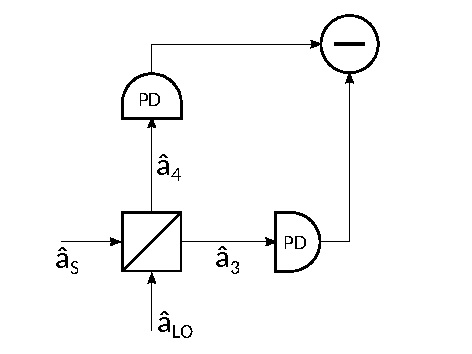
\includegraphics{../figures/scheme_homodyne.pdf}
%\caption{Balanced double homodyne detection.}
\end{figure}

This technique basically measures the phase difference between a input signal $S$ and a local oscillator $LO$. Figure xx shows the quantum mechanical description of the technique, in which $\hat{m}$ is the operator of the output difference between the photocurrents.\\


%--------------------------------------------------------------------------------------------------
%------------ SLIDE-------
\mysection{Homodyne Detection}\large
\vspace{0cm}

Given the input signal given by the state $\ket{\alpha}$ ($\alpha = |\alpha| e^{i\theta_\alpha}$) and the local oscillator given by state  $\ket{\beta}$ ($\beta = |\beta| e^{i\theta_\beta}$), the expected value of $\hat{m}$ and it's variance will be
%
\vspace{1em}
\begin{center}
	\begin{minipage}{85mm}
		\noindent
		\begin{equation}
			\braket{m} = 2|\alpha||\beta|\cos({\theta_\alpha - \theta_\beta})
		\end{equation}
	\end{minipage}
	$,\quad$
	\begin{minipage}{70mm}
		\noindent
		\begin{equation}
			\textrm{Var}(m) = |\alpha|^2 + |\beta|^2
		\end{equation}
	\end{minipage}
\end{center}
\vspace{1em}
%
If we normalize the units of $m$ by $2|\beta|$ and knowing that $\alpha \ll \beta$, then it can be simplified to
%
\vspace{1em}
\begin{center}
	\begin{minipage}{75mm}
		\noindent
		\begin{equation}
			\braket{m} = |\alpha|\cos({\theta_\alpha - \theta_\beta})
		\end{equation}
	\end{minipage}
	$,\quad$
	\begin{minipage}{45mm}
		\noindent
		\begin{equation}
			\textrm{Var}(m) \approx \frac{1}{4}
		\end{equation}
	\end{minipage}
\end{center}
%



%--------------------------------------------------------------------------------------------------
%------------ SLIDE-------
\mysection{Double Homodyne Detection}\large
\vspace{0cm}


In fact, we can measure the two quadratures $X$ and $Y$ at the same time, using the double homodyne detection. This tecnique consists in simply divide the signal in two beams with half the power of the original one and one of them is measure in-phase with the local oscillator, and the other is measured with a phase difference of $\pi/2$ relative to the first one???????
%
\begin{center}
	\begin{minipage}{85mm}
		\noindent
		\begin{equation}
			\braket{m_X} = \left|\frac{\alpha}{\sqrt{2}}\right| \cos({\theta_\alpha - \theta_\beta})
		\end{equation}
	\end{minipage}
	$,\quad$
	\begin{minipage}{50mm}
		\noindent
		\begin{equation}
			\textrm{Var}(m_X) \approx \frac{1}{4}
		\end{equation}
	\end{minipage}
\end{center}
%
%
\begin{center}
	\begin{minipage}{80mm}
		\noindent
		\begin{equation}
			\braket{m_Y} =  \left|\frac{\alpha}{\sqrt{2}}\right| \sin({\theta_\alpha - \theta_\beta})
		\end{equation}
	\end{minipage}
	$,\quad$
	\begin{minipage}{50mm}
		\noindent
		\begin{equation}
			\textrm{Var}(m_Y) \approx \frac{1}{4}
		\end{equation}
	\end{minipage}
\end{center}
%




%--------------------------------------------------------------------------------------------------
%------------ SLIDE-------
\mysection{Simulation setup}\large
\vspace{0cm}

\begin{figure}[h]
\label{fig:scheme_homodyne}
\centering
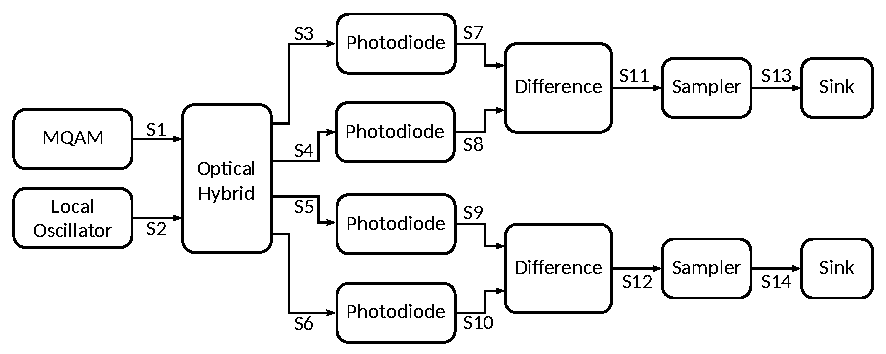
\includegraphics[width=\textwidth]{../figures/scheme_setup.pdf}
%\caption{Balanced double homodyne detection.}
\end{figure}

A state is generated in the MQAM which is then mixed in the Optical hybrid with a local oscillator. The 2 pairs of output optical signals are then converted to photocurrents. The difference between the signals of each pair is obtained and then is sampled.




%--------------------------------------------------------------------------------------------------
%------------ SLIDE-------
\mysection{Simulation results}\large
\vspace{0cm}

\begin{figure}[h]
\centering
	\begin{subfigure}
%		\label{fig:scheme_homodyne}
		\centering
		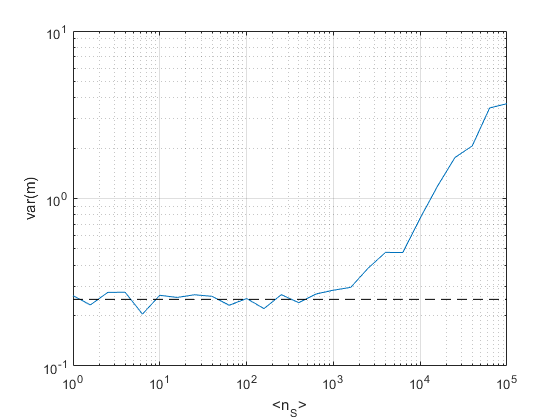
\includegraphics[height=65mm]{../figures/plot_var_vs_n1.png}
		%\caption{Balanced double homodyne detection.}
	\end{subfigure}
	\begin{subfigure}
%		\label{fig:scheme_homodyne}
		\centering
		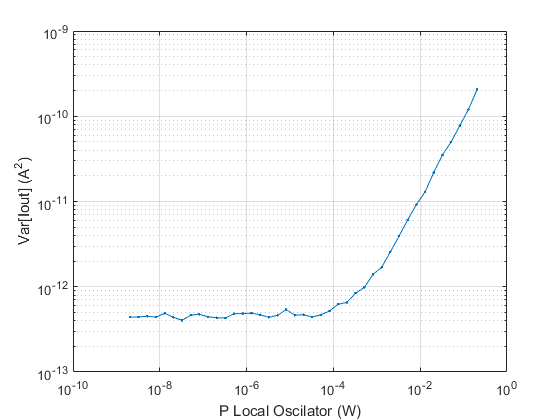
\includegraphics[height=65mm]{../figures/power_plot.png}
		%\caption{Balanced double homodyne detection.}
	\end{subfigure}
\end{figure}

These plots show the variance of $\hat{m}$ in function of signal power (left) and local oscillator power (right).



%--------------------------------------------------------------------------------------------------
%------------ SLIDE-------
\mysection{Experimental results}\large
\vspace{0cm}

\begin{figure}[h]
\centering
	\begin{subfigure}
%		\label{fig:scheme_homodyne}
		\centering
		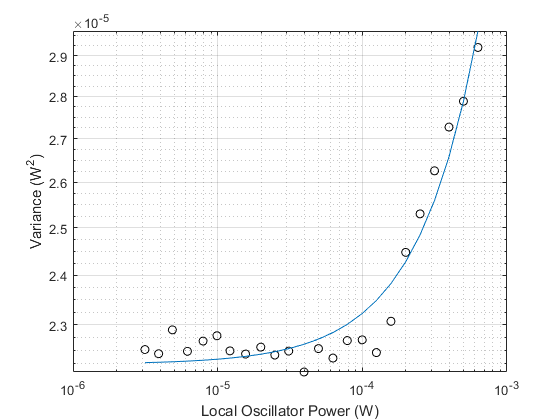
\includegraphics[height=65mm]{../figures/noise_exp_channel1.png}
		%\caption{Balanced double homodyne detection.}
	\end{subfigure}
	\begin{subfigure}
%		\label{fig:scheme_homodyne}
		\centering
		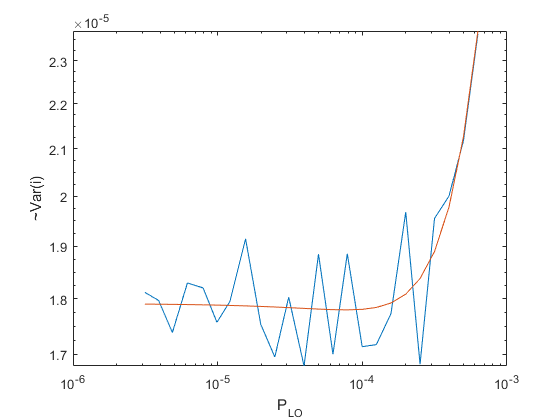
\includegraphics[height=65mm]{../figures/noise_exp_channel3.png}
		%\caption{Balanced double homodyne detection.}
	\end{subfigure}
\end{figure}

These plots show the experimental variance of a homodyne detection only with local oscillator, for two different quadratures and a degree 2 polynomial fitting.



%-------------------------------------------------------------------
%------------ SLIDE ------------------------------------------------
\mysection{} \sffamily
\vspace{-10mm}
\large\centerline{E-mail: diamantinosilva@ua.pt}


\end{document}
